\section{Esercitazione 4}

\subsection{Implementazione dei metodi diretti per sistemi lineari: fattorizzazione LU; pivoting}

Il metodo di eliminazione gaussiana, per la risoluzione di un sistema di equazioni lineari, si basa sull'idea di ridurre il sistema $A*x = b$ in un sistema equivalente (cioè avente soluzione identica) della forma $U*x = y$, dove U è una matrice triangolare superiore, e di risolvere questo sistema mediante sostituzioni all'indietro. Per rendersene conto, leggere ed eseguire il seguente m-file:

\lstinputlisting[style=customat, caption=Eliminazione Gaussiana]{../Esercitazione4/eliminazione_gaussiana.m}

Vediamo con un esempio come l'algoritmo appena mostrato sia equivalente ad una fattorizzazione $A=L*U$, seguita dalla soluzione dei due sistemi triangolari (rispettivamente inferiore e superiore) $L*y=b$ e $U*x=y$. Infatti, consideriamo il sistema $A*x = b$, e:

\begin{itemize} 

\item Sostituiamo ad A la sua fattorizzazione $L*U$, ovvero vale $A = L*U$, e quindi il sistema diventa: $L*U*x = b$; 
\item Poniamo  $U*x = y$, che è un sistema lineare a matrice triangolare superiore, da cui risulta $L*y = b$, che è un sistema lineare a matrice triangolare superiore; 
\item Ci ricaviamo y, conoscendo L e b, risolvendo il sistema lineare $L*y = b$ mediante semplici sostituzioni in avanti; 
\item Ci ricaviamo x, conoscendo U ed y, risolvendo il sistema lineare $U*x = y$ mediante semplici sostituzioni all'indietro.

\end{itemize}

Leggere ed eseguire il seguente m-file:   

\lstinputlisting[style=customat, caption=Esempio di fattorizzazione LU]{../Esercitazione4/EG_equiv_fattLU.m}

Esistono varie implementazioni possibili della fattorizzazione LU. Ad esempio le implementazioni degli algoritmi ``kji'' e ``ijk'' sono contenute nel codice seguente:

\lstinputlisting[style=customat, caption=Esempio di fattorizzazione LU]{../Esercitazione4/fattorizzazioni_LU_e_Cholesky.m}.

\subsection{Esercizio 1}

Guardare il codice sorgente delle due fattorizzazioni ``kji'' e ``ijk'' nel codice appena citato. Sapreste dire quale dei due accede per righe e quale per colonne?

\textbf{Risposta}:

\subsection{La tecnica del pivoting}

Per evitare di trovarsi un elemento pivotale nullo o molto piccolo, entrambe situazioni da evitare, in certe matrici è necessario applicare la tecnica del ``pivoting'', che vediamo spiegata nella figura seguente, rispettivamente per il pivoting parziale sulle righe (sinistra) e per il pivoting totale (destra):

\begin{figure}
\centering
\begin{subfigure}{.5\textwidth}
  \centering
  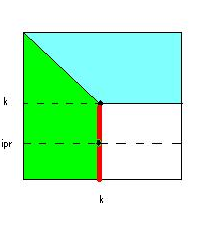
\includegraphics[width=.7\linewidth]{../Esercitazione4/images/figura_pivoting.png}
  \caption{Pivotint parziale sulle righe}
  \label{fig:pivoting1}
\end{subfigure}%
\begin{subfigure}{.5\textwidth}
  \centering
  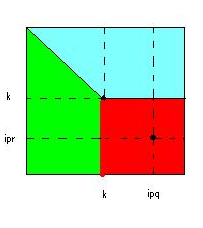
\includegraphics[width=.7\linewidth]{../Esercitazione4/images/figura_pivoting_1.png}
  \caption{Pivoting totale}
  \label{fig:pivoting2}
\end{subfigure}
\caption{Tecnica del Pivoting}
\label{fig:pivoting}
\end{figure}

dove l'elemento $(k,k)$ è il pivot ``naturale'', mentre $(ipr,k)$ e $(ipr,ipq)$ sono quelli determinati per ricerca del massimo valore nelle rispettive zone colorate di rosso:

\begin{itemize}

\item Per il pivoting parziale per righe la zona in rosso è la porzione di colonna di indici $(k:n,k)$;
\item Per il pivoting totale la zona in rosso è la sotto-matrice di indici $(k:n,k:n)$.

\end{itemize}

Una volta determinato l'elemento pivotale si procede allo scambio di righe/colonne:

\begin{itemize}

\item Si scambiano le righe ``k'' ed ``ipr'' nel pivoting parziale per righe;
\item Si scambiano le righe ``k'' ed ``ipr'' e le colonne ``k'' ed ``ipq'' nel pivoting totale;

\end{itemize}

Leggere ed eseguire il seguente m-file che implementa il pivoting parziale (sulle righe):

\lstinputlisting[style=customat, caption=Pivoting parziale]{../Esercitazione4/LU_con_pivoting_su_righe.m}

\subsection{Esercizio 2}  

Scrivere un programma Matlab/Octave che esegua la fattorizzazione LU con il pivoting totale e provarlo su una matrice piccola (ad es. 5x5, in modo da poterla visualizzare facilmente). Come verifica della correttezza dell'algoritmo implementato nel programma, si può verificare che $sum(sum(abs(A - L*U)))$ dia un valore molto piccolo.

\lstinputlisting[style=customat, caption=Fattorizzazione LU con pivoting totale]{../Esercitazione4/esercizio2.m}
